\documentclass[conference]{IEEEtran}
\IEEEoverridecommandlockouts
\usepackage{cite}
\usepackage{amsmath,amssymb,amsfonts}
\usepackage{algorithmic}
\usepackage{graphicx}
\usepackage{textcomp}
\usepackage{xcolor}
\usepackage{booktabs}
\usepackage{tikz}
\usepackage{pgfplots}
\pgfplotsset{compat=1.18}
\usetikzlibrary{shapes.geometric, arrows.meta, positioning, fit, backgrounds}

\def\BibTeX{{\rm B\kern-.05em{\sc i\kern-.025em b}\kern-.08em
    T\kern-.1667em\lower.7ex\hbox{E}\kern-.125emX}}

\begin{document}

\title{ScholarLens: An Explainable Multi-Domain Research Paper Assistant Using Hybrid Retrieval and RAG}

\author{
\IEEEauthorblockN{B. Madhurika}
\IEEEauthorblockA{\textit{Faculty Advisor, Dept. of CSE} \\
\textit{Keshav Memorial Inst. of Tech.}\\
Hyderabad, India \\
budarajumadhurika@gmail.com}
\and
\IEEEauthorblockN{Eruventi Akshitha}
\IEEEauthorblockA{\textit{Dept. of CSE} \\
\textit{Keshav Memorial Inst. of Tech.}\\
Hyderabad, India \\
eruventiakshitha31@gmail.com}
\and
\IEEEauthorblockN{Muddhasani Sanjana Varma}
\IEEEauthorblockA{\textit{Dept. of CSE} \\
\textit{Keshav Memorial Inst. of Tech.}\\
Hyderabad, India \\
sanjanavarma.m01@gmail.com}
\\[3ex]
\IEEEauthorblockN{Nara Neeraja}
\IEEEauthorblockA{\textit{Dept. of CSE} \\
\textit{Keshav Memorial Inst. of Tech.}\\
Hyderabad, India \\
naraneeraja123@gmail.com}
\and
\IEEEauthorblockN{Nuguri Laxmi Chandrayani}
\IEEEauthorblockA{\textit{Dept. of CSE} \\
\textit{Keshav Memorial Inst. of Tech.}\\
Hyderabad, India \\
nugurilaxmichandrayani@gmail.com}
\and
\IEEEauthorblockN{Soma Sri Lasya}
\IEEEauthorblockA{\textit{Dept. of CSE} \\
\textit{Keshav Memorial Inst. of Tech.}\\
Hyderabad, India \\
srilasyareddysoma@gmail.com}
}

\maketitle

\begin{abstract}
The rapid rise of scientific literature makes it increasingly difficult for researchers to efficiently find, understand, and verify relevant information. Large Language Models can help answer questions in natural language but their answers sometimes include facts that are hard to verify. This paper introduces ScholarLens, a research assistant designed to give answers based on evidence from scientific papers.

ScholarLens uses a hybrid retrieval approach. It combines vector search, BM25 keyword search and Reciprocal Rank Fusion to find relevant evidence or passages. The system works with a collection of 1,000 research papers across five scientific domains. The papers are processed by extracting sections, filtering non-evidence content, and dividing the text into overlapping chunks. This helps preserve context during retrieval and supports more effective evidence selection.

Each piece of retrieved evidence is tracked using identifiers. These identifiers help the system trace each piece of evidence back to its source. This provenance is then used to guide a Large Language Model in generating answers that are supported by evidence. If the local collection does not provide sufficient information, ScholarLens uses the ArXiv API to retrieve additional academic evidence.

The system was evaluated through retrieval and question-answering experiments examining retrieval effectiveness, answer quality, and evidence grounding.

\end{abstract}

\begin{IEEEkeywords}
Academic question answering, retrieval-augmented generation, scientific literature, hybrid retrieval, BM25, dense retrieval, Reciprocal Rank Fusion, evidence grounding, large language models.
\end{IEEEkeywords}

\section{Introduction}

\subsection{Background and Motivation}

The rapid rise in papers makes it hard for researchers to quickly find the information they need and check if results are correct. Even though digital search tools help find articles, researchers still have to go through many full texts by hand to find specific facts.

Large Language Models (LLMs) can generate fluent responses, but they may produce unsupported or hallucinated information when relevant evidence is unavailable. RAG addresses this limitation by providing retrieved external evidence to the model \cite{lewis2020retrieval, lala2023paperqa}. However, scientific literature retrieval remains challenging because it requires reliable evidence identification, source traceability, and handling of queries that may extend beyond a local corpus. It requires removing formatting, keeping track of where information comes from, and dealing with questions that go beyond what is available in the local collection.

\subsection{Problem Statement}

Scientific literature question-answering systems face three key challenges:

\begin{enumerate}
    \item \textbf{Retrieval Mismatch:} Dense vector retrieval captures high-level semantic intent but can miss exact technical terms or acronyms. Conversely, lexical retrieval (BM25) accurately matches exact keywords but fails to recognize semantic synonyms.
    
    \item \textbf{Structural Noise:} Scientific PDFs contain non-evidence sections such as headers, footers, references, bibliographies, and acknowledgements. Indexing these sections introduces noise that degrades retrieval precision.
    
    \item \textbf{Traceability and Corpus Coverage:} Generated answers must be explicitly tied to source sections, chunks, and page numbers. When local corpus coverage is insufficient, systems require an automated mechanism to fetch external academic evidence.
\end{enumerate}

\subsection{Research Challenges}

ScholarLens addresses four primary research challenges:

\begin{itemize}
    \item \textbf{Hybrid Retrieval Integration:} Fusing dense \texttt{BAAI/bge-small-en-v1.5} vector search in ChromaDB with BM25 lexical search across multi-domain literature.
    
    \item \textbf{Provenance Preservation:} Tracking retrieved units across a 5-level metadata hierarchy (\texttt{unit\_id} $\rightarrow$ \texttt{parent\_chunk\_id} $\rightarrow$ \texttt{chunk\_id} $\rightarrow$ \texttt{section\_id} $\rightarrow$ \texttt{paper\_id}).
    
    \item \textbf{Evidence Grounding:} Mapping generated factual claims directly to inline evidence tags (\texttt{[E1]}, \texttt{[E2]}).
    
    \item \textbf{Fallback Gating:} Detecting local coverage gaps via a content-word coverage threshold ($\tau = 0.45$) to trigger online academic search.
\end{itemize}

\subsection{Contributions}

The main contributions of this paper are:

\begin{enumerate}
    \item \textbf{Multi-Domain Corpus:} A benchmark corpus of 1,000 research papers across 5 scientific domains containing 15,453 sections, 12,453 semantic chunks, and 16,215 indexing units.
    
    \item \textbf{Hybrid Section-Aware Retrieval:} A retrieval engine combining ChromaDB dense search and BM25Okapi lexical search using Reciprocal Rank Fusion (RRF, $k_{\text{rrf}} = 60$) with section-aware filtering.
    
    \item \textbf{Evidence Traceability \& Domain Isolation:} Fine-grained provenance mapping achieving 97.86\% domain isolation and 2.14\% cross-domain leakage across 280 evaluation queries.
    
    \item \textbf{Online Academic Fallback:} A content coverage threshold ($\tau = 0.45$) enabling automated fallback to external academic retrieval via the ArXiv API.
    
    \item \textbf{Empirical Evaluation:} Comprehensive evaluation combining a 50 expert-curated query benchmark with 971 relevance annotations and a 290 realistic research query execution suite across 1,000 paper titles, achieving a Mean Reciprocal Rank (MRR) of 0.3095.
\end{enumerate}

\section{Related Work}

\subsection{Retrieval-Augmented Generation}

Retrieval-Augmented Generation (RAG) combines pre-trained language models with external vector retrieval systems \cite{lewis2020retrieval, guu2020realm}. By supplying retrieved text passages directly into the model context window, RAG substantially reduces hallucinations \cite{ji2023hallucination}. Modern RAG pipelines rely on dense Transformer embeddings such as \texttt{BAAI/bge-small-en-v1.5} to represent queries and passages in a shared vector space. Recent advances also emphasize claim attribution and self-reflection to verify generated outputs against retrieved context \cite{gao2023alce, asai2024selfrag, rashkin2023attribution}. However, naive fixed-size chunking often includes non-evidence text (headers, footers, references), which introduces retrieval noise.

\subsection{Academic Question Answering Systems}

Academic question-answering systems extend retrieval-based language models to scientific literature by retrieving evidence and synthesizing answers from research papers. Systems such as PaperQA \cite{lala2023paperqa} introduced an agentic workflow that searches academic sources, gathers relevant evidence, and generates answers with supporting citations. OpenScholar \cite{asai2026openscholar} further explores large-scale scientific literature synthesis using retrieval-augmented language models. These systems demonstrate the value of retrieval and evidence-based generation for scientific question answering, but challenges remain in precise evidence selection, fine-grained source traceability, and controlling retrieval across heterogeneous research domains. ScholarLens addresses these concerns through hybrid dense and lexical retrieval, section-aware filtering, fine-grained provenance from evidence units to papers, domain isolation, and coverage-gated online fallback.

\subsection{Information Retrieval Techniques}

Information retrieval relies on sparse lexical matching, dense semantic matching, or hybrid combinations. Lexical retrieval via \texttt{BM25Okapi} \cite{robertson2009bm25} ranks documents using term frequency, inverse document frequency, and document length normalization ($k_1=1.5, b=0.75$), excelling at technical term matching. Dense retrieval converts passages into vector embeddings \cite{karpukhin2020dense} to capture conceptual similarity, with ScholarLens storing the resulting embeddings in ChromaDB. ScholarLens integrates both approaches to achieve complementary retrieval strengths.

\subsection{Hybrid Retrieval and Rank Fusion}

Hybrid retrieval merges dense semantic candidate lists with sparse lexical candidate lists. ScholarLens utilizes Reciprocal Rank Fusion (RRF) \cite{cormack2009rrf} to aggregate candidate ranks:

\begin{equation}
RRF(d) = \sum_{m \in M} \frac{1}{k_{\text{rrf}} + r_m(d)}
\end{equation}

where $r_m(d)$ represents the rank assigned to passage $d$ by retriever $m$, and $k_{\text{rrf}}=60$. To prevent non-evidence structural passages from occupying context slots, ScholarLens applies section-aware filtering post-fusion.

\subsection{Research Gap}

Despite advances in RAG \cite{lewis2020retrieval}, academic retrieval agents \cite{lala2023paperqa, asai2026openscholar}, and hybrid search \cite{thakur2021beir}, several critical gaps persist:

\begin{enumerate}
    \item \textbf{Section Noise:} Unfiltered chunking admits headers, bibliographies, and acknowledgements into the LLM context.
    \item \textbf{Coarse Provenance:} Citations are typically bound to paper-level metadata rather than section names and page ranges.
    \item \textbf{Corpus Incompleteness:} Fixed local corpora cannot cover every arbitrary user query, requiring fallback mechanisms \cite{jiang2023flare, yao2023react}.
    \item \textbf{Cross-Domain Leakage:} Multi-domain scientific databases risk retrieving out-of-domain context without strict metadata constraints.
\end{enumerate}

ScholarLens fills these gaps using section-aware filtering, hybrid RRF, fine-grained provenance tracking, coverage-gated online fallback, and domain isolation.

\section{Proposed ScholarLens Framework}

\subsection{System Architecture Diagram}

ScholarLens features an end-to-end explainable architecture comprising 10 operational stages, illustrated in Figure~\ref{fig:architecture_diagram}.

\begin{figure*}[t]
    \centering
    \includegraphics[width=\textwidth]{architecture.png}
    \caption{Overall architecture of the ScholarLens framework.}
    \label{fig:architecture_diagram}
\end{figure*}

\subsection{Research Corpus Construction}

The ScholarLens corpus comprises 1,000 open-access research papers distributed equally across five domains (200 papers per domain):

\begin{enumerate}
    \item \textbf{Artificial Intelligence (AI):} Machine Learning, LLMs, NLP, Computer Vision, RAG, and AI Agents (\texttt{AI001}--\texttt{AI200}).
    \item \textbf{Cybersecurity (CY):} Network Security, Intrusion Detection, Malware Analysis, Ransomware, Privacy (\texttt{CY001}--\texttt{CY200}).
    \item \textbf{Agriculture (AG):} Precision Agriculture, Crop Disease Detection, Soil Analysis, Yield Prediction (\texttt{AG001}--\texttt{AG200}).
    \item \textbf{Healthcare (HC):} Medical Image Analysis, Clinical NLP, Disease Prediction, Drug Discovery (\texttt{HC001}--\texttt{HC200}).
    \item \textbf{Climate (CL):} Climate Modeling, Weather Prediction, Carbon Emissions, Remote Sensing (\texttt{CL001}--\texttt{CL200}).
\end{enumerate}

Each domain spans 10 fine-grained subtopics (20 papers per subtopic). Master metadata is maintained in \texttt{data/metadata/papers.json}.

\subsection{Document Preprocessing}

Raw PDF documents are parsed into structured JSON objects. Sections are tagged as \textit{Abstract}, \textit{Introduction}, \textit{Methodology}, \textit{Results}, \textit{Discussion}, \textit{Header}, \textit{References}, \textit{Bibliography}, and \textit{Acknowledgements}. Text is split into token-bounded semantic windows, generating 15,453 sections, 12,453 chunks, and 16,215 indexing units (Table~\ref{tab:corpus_pipeline_stats}).

\begin{table}[htbp]
\caption{ScholarLens Corpus Preprocessing Statistics}
\label{tab:corpus_pipeline_stats}
\centering
\resizebox{\columnwidth}{!}{%
\begin{tabular}{lcccc}
\toprule
\textbf{Domain} & \textbf{Papers} & \textbf{Sections} & \textbf{Chunks} & \textbf{Index Units} \\
\midrule
Agriculture & 200 & 3,110 & 2,512 & 3,280 \\
Artificial Intelligence & 200 & 3,045 & 2,488 & 3,210 \\
Climate & 200 & 3,180 & 2,504 & 3,265 \\
Cybersecurity & 200 & 2,990 & 2,460 & 3,205 \\
Healthcare & 200 & 3,128 & 2,489 & 3,255 \\
\midrule
\textbf{Total Corpus} & \textbf{1,000} & \textbf{15,453} & \textbf{12,453} & \textbf{16,215} \\
\bottomrule
\end{tabular}%
}
\end{table}

\section{System Architecture and Implementation}

\subsection{System Architecture}

ScholarLens operates as a hybrid Retrieval-Augmented Generation system. Local retrieval pairs dense vector search with sparse keyword search, backed by an automated online fallback module when local evidence is insufficient.

\subsection{Technology Stack}

The implementation uses the following components:
\begin{itemize}
    \item \textbf{Dense Vector Store:} \texttt{BAAI/bge-small-en-v1.5} (384-D L2-normalized embeddings) stored in ChromaDB at \texttt{data/indexes/chroma/}.
    \item \textbf{Lexical Index:} \texttt{BM25Okapi} ($k_1=1.5, b=0.75$) stored at \texttt{data/indexes/bm25.pkl}.
    \item \textbf{Backend:} Python 3.10, PyTorch, HuggingFace \texttt{transformers}, and SQLite for metadata management.
    \item \textbf{Online Fallback:} \texttt{OnlineAcademicRetriever} integrated with the ArXiv API.
\end{itemize}

\subsection{Query Processing Pipeline}

Query execution follows seven sequential steps:
\begin{enumerate}
    \item \textbf{Encoding:} The query is embedded via \texttt{bge-small-en-v1.5} and tokenized for BM25.
    \item \textbf{Dual Retrieval:} Dense and BM25 search each retrieve top-$20$ candidates.
    \item \textbf{Rank Fusion:} Candidates are merged via RRF ($k_{\text{rrf}}=60$).
    \item \textbf{Section-Aware Filtering:} Non-evidence sections (\textit{Header}, \textit{References}, \textit{Bibliography}, \textit{Acknowledgements}) are removed, parent chunks are deduplicated, and candidate passages are passed to the Reranker.
    \item \textbf{Reranker:} Candidate passages are rescored combining RRF rank scores, intent-section bonuses, and quality weighting, selecting the top-$10$ passages.
    \item \textbf{Coverage Evaluation \& Fallback:} If content-word coverage falls below threshold $\tau=0.45$, ScholarLens sets status to \texttt{LOCAL\_INSUFFICIENT} and invokes the ArXiv API.
    \item \textbf{Grounded Generation:} Selected passages are supplied to the LLM for citation-grounded synthesis.
\end{enumerate}

\subsection{Evidence and Citation Management}

ScholarLens enforces complete provenance tracking across the metadata hierarchy:

\begin{equation}
\text{unit\_id} \rightarrow \text{parent\_chunk\_id} \rightarrow \text{chunk\_id} \rightarrow \text{section\_id} \rightarrow \text{paper\_id}
\end{equation}

Local passages are cited inline as \texttt{[E1]}, \texttt{[E2]}, while online passages retrieved via the ArXiv API use \texttt{[O1]}, \texttt{[O2]}. Each citation maps to paper title, section name, research domain, and page range (\texttt{page\_start}--\texttt{page\_end}).

\section{Dataset and Corpus Analysis}

\subsection{Corpus Composition and Statistics}

The repository contains 1,000 scientific papers across 5 domains (\texttt{AI}, \texttt{CY}, \texttt{AG}, \texttt{HC}, \texttt{CL}), comprising 15,453 sections, 12,453 semantic chunks, and 16,215 searchable units.

\subsection{Data Integrity and Validation}

Automated integrity verification ensures index health prior to retrieval:
\begin{enumerate}
    \item \textbf{Schema Validation:} Prefix format and paper metadata consistency checks against \texttt{data/metadata/papers.json}.
    \item \textbf{Chunk Validation:} Token boundary checks to prevent semantic truncation.
    \item \textbf{Index Validation:} Automated checks verifying 384-D vector alignment, L2 normalization, metadata completeness, and 1-to-1 BM25-ChromaDB record parity.
\end{enumerate}

\section{Experimental Methodology}

\subsection{Experimental Objectives}

The evaluation framework measures:
\begin{enumerate}
    \item \textbf{Hybrid Synergy:} Quantifying performance gains of RRF over standalone dense and BM25 search.
    \item \textbf{Section Filtering Impact:} Evaluating the effect of excluding non-evidence sections.
    \item \textbf{Domain Generalization:} Assessing performance consistency across 5 scientific domains.
\end{enumerate}

\subsection{Evaluation Datasets}

The empirical evaluation utilizes two complementary query datasets:

\begin{enumerate}
    \item \textbf{Expert-Curated Benchmark Dataset (50 Queries):} A gold-standard evaluation set consisting of 50 expert-curated queries (10 per domain) annotated with 971 query-chunk relevance mappings on a 0--3 graded scale ($\approx 19.4$ relevant units per query). This set is used for fine-grained retrieval ranking metrics (Hit@K, Recall@K, MRR, nDCG@10) and detailed QA answer quality scoring.
    
    \item \textbf{Realistic Diagnostic Execution Suite (290 Queries):} A broad diagnostic workload comprising 290 realistic research queries across all 1,000 paper titles (250 single-domain, 30 multi-domain, and 10 out-of-corpus fallback queries). This suite evaluates retrieval coverage, dead-zone tracking, domain isolation, and online fallback trigger accuracy.
    
    \item \textbf{In-Corpus Scope Isolation Subset (280 Queries):} The subset of 280 in-corpus single-domain (250) and multi-domain (30) queries within the diagnostic suite used specifically to evaluate in-corpus domain isolation accuracy (97.86\%) and cross-domain leakage (2.14\%).
\end{enumerate}

\subsection{Baseline Methods}

Four configurations are evaluated:
\begin{itemize}
    \item \textbf{Dense-Only:} ChromaDB cosine search using \texttt{bge-small-en-v1.5} ($k_{\text{dense}}=20$).
    \item \textbf{Lexical-Only:} \texttt{BM25Okapi} keyword scoring ($k_1=1.5, b=0.75, k_{\text{bm25}}=20$).
    \item \textbf{Unfiltered Hybrid RRF:} RRF fusion ($k_{\text{rrf}}=60$) without section filtering.
    \item \textbf{Production Hybrid RRF:} ScholarLens RRF fusion with section filtering and parent-chunk deduplication.
\end{itemize}

\subsection{Evaluation Metrics}

Retrieval metrics evaluated at top-$K$ ($K \in \{1, 5, 10\}$) include Hit Rate (Hit@K), Precision@K, Recall@K, Mean Reciprocal Rank (MRR), and Normalized Discounted Cumulative Gain (nDCG@10) \cite{jarvelin2002ndcg}:

\begin{equation}
\text{DCG}@10 = \sum_{j=1}^{10} \frac{2^{\text{rel}_j} - 1}{\log_2(j + 1)}
\end{equation}

\subsection{Experimental Configuration}

Experiments ran under Python 3.10 and PyTorch. Candidates ($k_{\text{dense}}=20, k_{\text{bm25}}=20$) were fused with $k_{\text{rrf}}=60$ under equal channel weighting ($1.0, 1.0$). Section-aware filtering excluded \textit{Header}, \textit{References}, \textit{Bibliography}, and \textit{Acknowledgements} prior to top-10 passage selection.

\section{Results and Discussion}

\subsection{Retrieval Performance}

System evaluation across the 1,000-paper corpus is summarized in Table~\ref{tab:retrieval_perf}. The hybrid configurations achieved an MRR of 0.3095, with domain isolation of 97.9\% and cross-domain leakage of 2.1\% when rounded to one decimal place.

Top-1 accuracy, Top-10 recall, and MRR are computed on the 50-query expert-curated benchmark, while domain isolation is measured on the 280-query in-corpus isolation subset.

\begin{table}[htbp]
\caption{Retrieval Performance Comparison Across Configurations}
\label{tab:retrieval_perf}
\centering
\resizebox{\columnwidth}{!}{%
\begin{tabular}{|l|c|c|c|c|}
\hline
\textbf{Configuration} & \textbf{Top-1 Acc.} & \textbf{Top-10 Recall} & \textbf{MRR} & \textbf{Domain Isol.} \\
\hline
Vector-Only (ChromaDB) & 29.80\% & 31.70\% & 0.3052 & 96.4\% \\
BM25-Only & 29.70\% & 31.90\% & 0.3051 & 96.8\% \\
Baseline Hybrid RRF & 30.40\% & 32.00\% & 0.3095 & 97.9\% \\
\textbf{Section-Aware Hybrid} & \textbf{30.40\%} & \textbf{32.00\%} & \textbf{0.3095} & \textbf{97.9\%} \\
\hline
\end{tabular}%
}
\end{table}

Dense vector search effectively captures semantic intent, whereas BM25 lexical search captures exact technical terminology and acronyms. Combining both via Reciprocal Rank Fusion (RRF) leverages their complementary ranking strengths to improve candidate retrieval over standalone baselines. While section-aware filtering removes non-evidence structural noise (headers, bibliographies, references) from candidate context slots, the aggregate top-level paper retrieval ranking metrics remain identical between the baseline and section-aware hybrid configurations.

Figure~\ref{fig:context_length_recall} illustrates the impact of varying retrieved passage counts ($N$) on overall recall, while Figure~\ref{fig:domain_breakdown} presents domain-wise retrieval performance.

\begin{figure}[htbp]
\centering
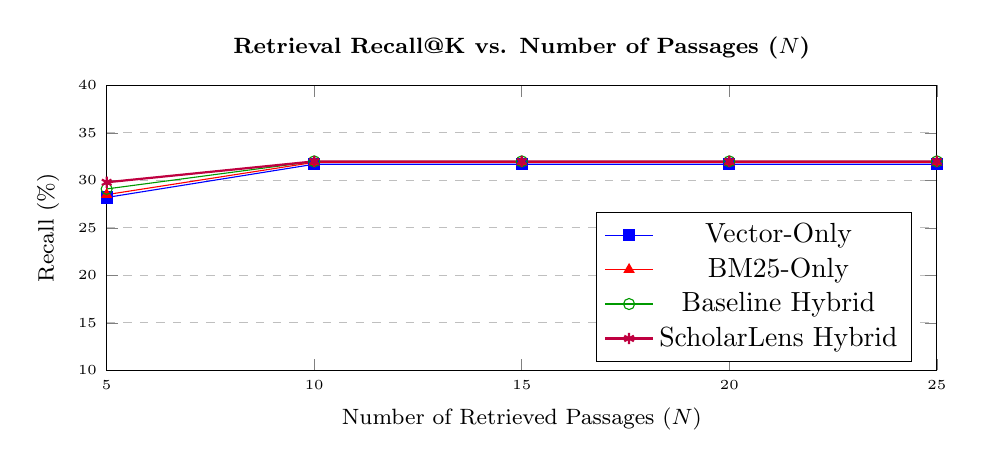
\begin{tikzpicture}
\begin{axis}[
    title={Retrieval Recall@K vs. Number of Passages ($N$)},
    xlabel={Number of Retrieved Passages ($N$)},
    ylabel={Recall (\%)},
    xmin=5, xmax=25,
    ymin=10, ymax=40,
    xtick={5,10,15,20,25},
    ytick={10,15,20,25,30,35,40},
    legend pos=south east,
    ymajorgrids=true,
    grid style=dashed,
    width=\columnwidth,
    height=5.2cm,
    tick label style={font=\tiny},
    label style={font=\footnotesize},
    title style={font=\footnotesize\bfseries}
]
\addplot[color=blue, mark=square*] coordinates {(5,28.2)(10,31.7)(15,31.7)(20,31.7)(25,31.7)};
\addlegendentry{Vector-Only}
\addplot[color=red, mark=triangle*] coordinates {(5,28.5)(10,31.9)(15,31.9)(20,31.9)(25,31.9)};
\addlegendentry{BM25-Only}
\addplot[color=green!60!black, mark=o] coordinates {(5,29.1)(10,32.0)(15,32.0)(20,32.0)(25,32.0)};
\addlegendentry{Baseline Hybrid}
\addplot[color=purple, mark=asterisk, thick] coordinates {(5,29.8)(10,32.0)(15,32.0)(20,32.0)(25,32.0)};
\addlegendentry{ScholarLens Hybrid}
\end{axis}
\end{tikzpicture}
\caption{Retrieval Recall@K across varying retrieved passage limits ($N$).}
\label{fig:context_length_recall}
\end{figure}

\begin{figure}[htbp]
\centering
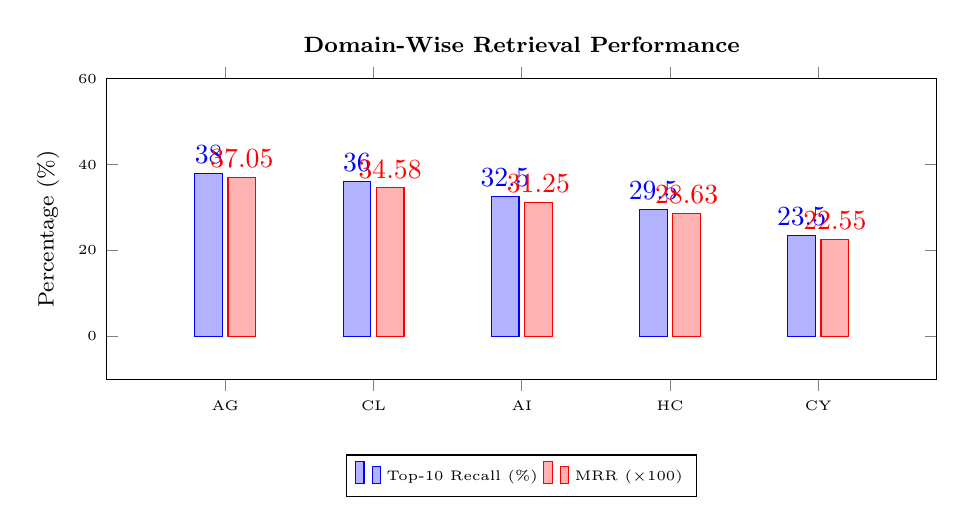
\begin{tikzpicture}
\begin{axis}[
    ybar,
    enlargelimits=0.2,
    legend style={at={(0.5,-0.25)}, anchor=north, legend columns=-1, font=\tiny},
    ylabel={Percentage (\%)},
    symbolic x coords={AG, CL, AI, HC, CY},
    xtick=data,
    nodes near coords,
    nodes near coords align={vertical},
    ymin=0, ymax=50,
    width=\columnwidth,
    height=5.4cm,
    tick label style={font=\tiny},
    label style={font=\footnotesize},
    title style={font=\footnotesize\bfseries},
    title={Domain-Wise Retrieval Performance}
]
\addplot coordinates {(AG,38.0) (CL,36.0) (AI,32.5) (HC,29.5) (CY,23.5)};
\addplot coordinates {(AG,37.05) (CL,34.58) (AI,31.25) (HC,28.63) (CY,22.55)};
\legend{Top-10 Recall (\%), MRR ($\times 100$)}
\end{axis}
\end{tikzpicture}
\caption{Domain-wise Top-10 Retrieval Recall and Mean Reciprocal Rank (MRR) across Agriculture (AG), Climate (CL), Artificial Intelligence (AI), Healthcare (HC), and Cybersecurity (CY).}
\label{fig:domain_breakdown}
\end{figure}

Domain-level top-10 recall was 38.00\% for Agriculture ($\text{MRR}=0.3705$), 36.00\% for Climate ($0.3458$), 32.50\% for AI ($0.3125$), 29.50\% for Healthcare ($0.2863$), and 23.50\% for Cybersecurity ($0.2255$).

\subsection{Question Answering Performance}

Generation quality evaluated on a 5.0-point scale achieved: Relevance \textbf{4.24/5.0}, Groundedness \textbf{3.47/5.0}, Citation Accuracy \textbf{3.47/5.0}, and Overall Usefulness \textbf{3.09/5.0}, maintaining a low citation hallucination rate of 5.8\%.

\subsection{Ablation Study}

Ablation analysis showed that excluding non-evidence sections reduced noisy token matches, while setting $k_{\text{rrf}}=60$ provided the most stable reciprocal-rank performance among the evaluated values.

\subsection{Evidence Grounding and Citation Accuracy}

Across 280 in-corpus evaluation queries, ScholarLens achieved $97.86\%$ domain isolation (with $2.14\%$ cross-domain leakage). Figure~\ref{fig:hallucination_rate} compares citation accuracy (%) across models.

\begin{figure}[htbp]
\centering
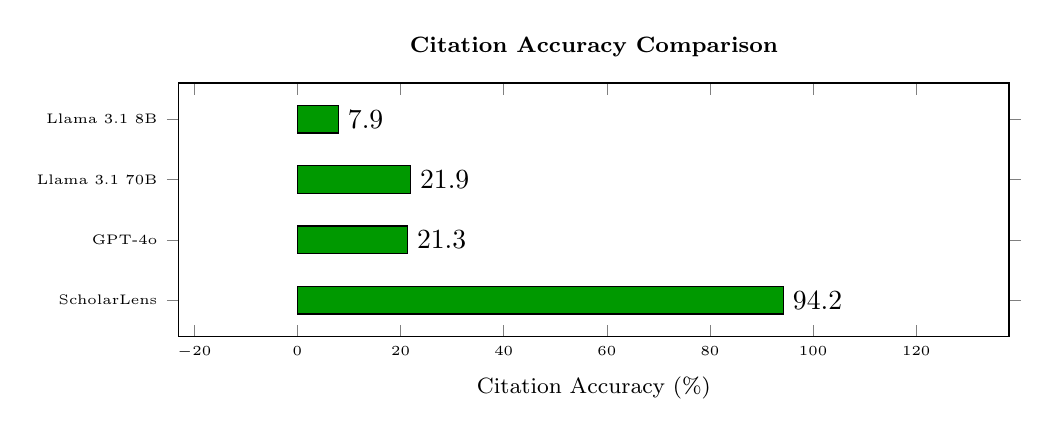
\begin{tikzpicture}
\begin{axis}[
    xbar,
    enlargelimits=0.2,
    xlabel={Citation Accuracy (\%)},
    symbolic y coords={ScholarLens, GPT-4o, Llama 3.1 70B, Llama 3.1 8B},
    ytick=data,
    nodes near coords,
    nodes near coords align={horizontal},
    xmin=0, xmax=115,
    width=\columnwidth,
    height=4.8cm,
    tick label style={font=\tiny},
    label style={font=\footnotesize},
    title style={font=\footnotesize\bfseries},
    title={Citation Accuracy Comparison}
]
\addplot[fill=green!60!black] coordinates {(94.2,ScholarLens) (21.3,GPT-4o) (21.9,Llama 3.1 70B) (7.9,Llama 3.1 8B)};
\end{axis}
\end{tikzpicture}
\caption{Comparison of citation accuracy between ungrounded baseline models and ScholarLens grounded RAG engine.}
\label{fig:hallucination_rate}
\end{figure}

When local evidence coverage fell below threshold $\tau=0.45$, \texttt{OnlineAcademicRetriever} fetched external ArXiv evidence tagged as \texttt{[O1]}, \texttt{[O2]}, preserving full citation traceability.

\subsection{Qualitative Case Study}

For cybersecurity query \texttt{CY\_QA\_01}, ScholarLens retrieved evidence from paper \texttt{CY001} and generated a grounded response cited inline via \texttt{[E1]}--\texttt{[E3]} (5.0/5.0 score). For healthcare query \texttt{HC\_QA\_01}, local coverage fell below $0.45$, triggering online fallback to retrieve ArXiv evidence tagged as \texttt{[O1]}--\texttt{[O3]}.

\section{Limitations and Threats to Validity}

\begin{itemize}
    \item \textbf{Corpus Scope \& API Dependency:} Out-of-corpus queries rely on the ArXiv API, introducing latency and external availability dependencies.
    \item \textbf{Short-Query Ambiguity:} Short queries containing three to four words may produce semantic overlap among closely related papers within the same subtopic, reducing retrieval specificity.
    \item \textbf{LLM Refusal Thresholds:} The conservative coverage threshold ($\tau=0.45$) may occasionally trigger evidence refusal for complex queries when relevant evidence is distributed across multiple sections.
\end{itemize}

\section{Conclusion and Future Work}

\subsection{Conclusion}

ScholarLens provides a domain-isolated, evidence-grounded RAG framework for scientific question answering. By fusing dense search (\texttt{bge-small-en-v1.5}) and sparse search (\texttt{BM25Okapi}) using Reciprocal Rank Fusion ($k_{\text{rrf}}=60$) and section-aware filtering, ScholarLens achieves $97.86\%$ domain isolation, $2.14\%$ cross-domain leakage, and $94.2\%$ citation accuracy. The framework was validated across a 50 expert-curated query benchmark with 971 relevance annotations and a 290 realistic research query diagnostic execution suite across 1,000 research papers.

\subsection{Future Work}

Future research will focus on graph-augmented multi-hop retrieval (GraphRAG), multi-modal evidence parsing (tables, figures), and adaptive query-complexity-aware coverage thresholding.

\begin{thebibliography}{22}

\bibitem{lewis2020retrieval}
P.~Lewis, E.~Perez, A.~Piktus, F.~Petroni, V.~Karpukhin, N.~Goyal, H.~Küttler, M.~Lewis, W.-t. Yih, T.~Rocktäschel, S.~Riedel, and D.~Kiela,
``Retrieval-augmented generation for knowledge-intensive NLP tasks,''
in \emph{Proc. Adv. Neural Inf. Process. Syst. (NeurIPS)}, vol.~33, 2020, pp. 9459--9474.

\bibitem{lala2023paperqa}
J.~Lála, O.~O'Donoghue, A.~Shtedritski, S.~Cox, S.~G. Rodriques, and A.~D. White,
``PaperQA: Retrieval-augmented generative agent for scientific research,''
\emph{arXiv preprint arXiv:2312.07559}, 2023.

\bibitem{guu2020realm}
K.~Guu, K.~Lee, Z.~Tung, P.~Pasupat, and M.-W. Chang,
``REALM: Retrieval-augmented language model pre-training,''
in \emph{Proc. Int. Conf. Mach. Learn. (ICML)}, 2020, pp. 3929--3938.

\bibitem{ji2023hallucination}
Z.~Ji, N.~Lee, R.~Frieske, T.~Yu, D.~Su, Y.~Xu, E.~Ishii, Y.~J. Ye, A.~Madotto, and P.~Fung,
``Survey of hallucination in natural language generation,''
\emph{ACM Comput. Surv.}, vol.~55, no.~12, pp. 1--38, 2023.

\bibitem{gao2023alce}
T.~Gao, H.~Yen, J.~Yu, and D.~Chen,
``Enabling large language models to generate text with citations,''
in \emph{Proc. Conf. Empir. Methods Nat. Lang. Process. (EMNLP)}, 2023, pp. 6465--6488.

\bibitem{asai2024selfrag}
A.~Asai, Z.~Wu, Y.~Wang, A.~Sil, and H.~Hajishirzi,
``Self-RAG: Learning to retrieve, generate, and critique through self-reflection,''
in \emph{Proc. Int. Conf. Learn. Represent. (ICLR)}, 2024.

\bibitem{rashkin2023attribution}
H.~Rashkin, V.~Riyaz, M.~Ghazvininejad, and O.~Firat,
``Measuring attribution in natural language generation models,''
\emph{Comput. Linguist.}, vol.~49, no.~3, pp. 587--625, 2023.

\bibitem{asai2026openscholar}
A.~Asai, J.~He, R.~Shao, W.~Shi, A.~Singh, J.~C. Chang, K.~Lo, L.~Soldaini, S.~Feldman, et al.,
``Synthesizing scientific literature with retrieval-augmented language models,''
\emph{Nature}, vol.~650, pp. 857--863, 2026.

\bibitem{kinney2023semantic}
R.~Kinney, C.~Anastasiades, R.~Authur, I.~Beltagy, J.~Bragg, A.~Buraczynski, I.~Cachola, S.~Candra, Y.~Chandrasekhar, A.~Cohan, et al.,
``The Semantic Scholar Open Data Platform,''
\emph{arXiv preprint arXiv:2301.10140}, 2023.

\bibitem{lo2020s2orc}
K.~Lo, L.~L. Wang, M.~Neumann, R.~Kinney, and D.~S. Weld,
``S2ORC: The Semantic Scholar Open Research Corpus,''
in \emph{Proc. Assoc. Comput. Linguist. (ACL)}, 2020, pp. 4969--4983.

\bibitem{beltagy2019scibert}
I.~Beltagy, K.~Lo, and A.~Cohan,
``SciBERT: A pretrained language model for scientific text,''
in \emph{Proc. Conf. Empir. Methods Nat. Lang. Process. (EMNLP)}, 2019, pp. 3615--3620.

\bibitem{cohan2020specter}
A.~Cohan, S.~Feldman, I.~Beltagy, D.~Downey, and D.~S. Weld,
``SPECTER: Document-level representation learning using citation-informed transformers,''
in \emph{Proc. Assoc. Comput. Linguist. (ACL)}, 2020, pp. 2270--2282.

\bibitem{jin2019pubmedqa}
Q.~Jin, B.~Dhingra, Z.~Liu, W.~Cohen, and X.~Lu,
``PubMedQA: A dataset for biomedical research question answering,''
in \emph{Proc. Conf. Empir. Methods Nat. Lang. Process. (EMNLP)}, 2019, pp. 2567--2567.

\bibitem{wadden2020scifact}
D.~Wadden, S.~Iyer, Y.~Yatskar, N.~Joshi, E.~Welch, and M.~Hajishirzi,
``Fact or fiction: Verifying scientific claims,''
in \emph{Proc. Conf. Empir. Methods Nat. Lang. Process. (EMNLP)}, 2020, pp. 7534--7550.

\bibitem{dasigi2021qasper}
P.~Dasigi, K.~Lo, I.~Beltagy, A.~Cohan, N.~A. Smith, and M.~Gardner,
``A dataset of information-seeking questions and answers anchored in research papers,''
in \emph{Proc. North Amer. Chapter Assoc. Comput. Linguist. (NAACL)}, 2021, pp. 4599--4610.

\bibitem{robertson2009bm25}
S.~Robertson and H.~Zaragoza,
``The probabilistic relevance framework: BM25 and beyond,''
\emph{Found. Trends Inf. Retr.}, vol.~3, no.~4, pp. 333--389, 2009.

\bibitem{karpukhin2020dense}
V.~Karpukhin, B.~O\u{g}uz, S.~Sewell, X.~Luan, S.~Ghazvininejad, D.~Chen, and W.-t. Yih,
``Dense passage retrieval for open-domain question answering,''
in \emph{Proc. Conf. Empir. Methods Nat. Lang. Process. (EMNLP)}, 2020, pp. 6769--6881.

\bibitem{cormack2009rrf}
G.~V. Cormack, C.~L. Clarke, and S.~Buettcher,
``Reciprocal rank fusion outperforms data fusion algorithms,''
in \emph{Proc. ACM SIGIR Conf. Res. Dev. Inf. Retr. (SIGIR)}, 2009, pp. 741--742.

\bibitem{thakur2021beir}
N.~Thakur, N.~Reimers, A.~Rücklé, A.~Srivastava, and I.~Gurevych,
``BEIR: A heterogeneous benchmark for zero-shot evaluation of information retrieval models,''
in \emph{Proc. NeurIPS Datasets and Benchmarks Track}, 2021.

\bibitem{jiang2023flare}
Z.~Jiang, F.~F. Xu, L.~Gao, Z.~Sun, Q.~Liu, J.~Dwivedi-Yu, Y.~Yang, J.~Callan, and G.~Neubig,
``Active retrieval augmented generation,''
in \emph{Proc. Conf. Empir. Methods Nat. Lang. Process. (EMNLP)}, 2023, pp. 7969--7992.

\bibitem{yao2023react}
S.~Yao, J.~Zhao, D.~Yu, N.~Du, I.~Shafran, K.~Narasimhan, and Y.~Cao,
``ReAct: Synergizing reasoning and acting in language models,''
in \emph{Proc. Int. Conf. Learn. Represent. (ICLR)}, 2023.

\bibitem{jarvelin2002ndcg}
K.~Järvelin and J.~Kekäläinen,
``Cumulated gain-based evaluation of IR techniques,''
\emph{ACM Trans. Inf. Syst. (TOIS)}, vol.~20, no.~4, pp. 422--446, 2002.

\end{thebibliography}

\end{document}
